\documentclass{article}
\usepackage{graphicx}
\usepackage{amsmath}
\usepackage{authblk}
\usepackage{tabu}
\newcommand{\newpar}{\vsapce{.2in}\noindent}
 \usepackage{booktabs}
 \usepackage{multirow}
\begin{document}

\title{A Proxemic Multimedia Interaction over the
Internet of Things}
\author{Pankaj Verma, Sanjay Meena, and Keshav Verma}
\affil{{CSPLab, Indian Institute of technology, Rupnagar,Punjab}}
\affil{{{aahma078,msain2,elsaddik}@uottawa.ca
http://www.mcrlab.uottawa.ca/}}
\maketitle

\begin
\noindent\textbf{Abstract.}With the rapid growth of online devices, a new concept of
Internet of Things (IoT) is emerging in which everyday devices will be
connected to the Internet. As the number of devices in IoT is increasing,
so is the complexity of the interactions between user and devices. There
is a need to design intelligent user interfaces that could assist users in
interactions. The present study proposes a proximity-based user inter-
face for multimedia devices over IoT. The proposed method employs a
cloud-based decision engine to support user to choose and interact with
the most appropriate device, reliving the user from the burden of enu-
merating available devices manually. The decision engine observes the
multimedia content and device properties, learns user preferences adap-
tively, and automatically recommends the most appropriate device to
interact. The system evaluation shows that the users agree with the pro-
posed interaction 70 \% of the times. 

\noindent\textbf{Keywords:}Proxemic interaction; multimedia interaction ; user inter-
face; elicitation study
\end

\section{Introduction}
The Internet has been expanding very rapidly with time. Now, more than 2.7
billion people (almost 39\% of world's population) have access to it and use it in their daily life[1]. The number of devices that are connected to the Internet has been growing dramatically. Therefore, a new concept of Internet of Things (IoT)is emerging[2]. More than 11.2 billion devices were connected to the Internet in 2013 and it is predicted that there will be around 50 billion devices online by 2020[3]. These uniquely identfiable objects and devices move and interact with each other to accomplish various tasks. In other words, IoT is like a big and dynamic society of objects and people. But we are far from the ubiquitous computing vision of Weiser [4] due to two main reasons: the lack of an appropriate task-centered User Interface (UI) design approach and the lack of reliable support for distributable user interfaces in ubiquitous environments [5]. Thus, there is a need for a new generation of specically designed user interfaces for IoT.

More than 7 billion people constantly use verbal and nonverbal communica-
tion techniques to interact with their society all across the world. Verbal communication is considered as the main channel since it is used explicitly. However,nonverbal communication such as Proxemics, Haptics, Body Language, etc. plays an important role in the human society because it uses implicit interactions. In the same way, nonverbal communication can also enhance the interactions within the IoT, which is ike human's society except the size of IoT is few times bigger than human society. Thus, nonverbal techniques should be used in order to build proper user interfaces for ubiquitous environments, particularly the IoT.

The present study proposes a distributed user interface that provides a suitable environment for multimedia interactions over the IoT. It consists of a cloud-based decision engine that manages the proxemic interactions. This engine is called Proxemic Interaction Unit (PIU). PIU uses multimedia devices within the IoT as elements of a universal UI in order to assist users to make use of their surrounding devices. We collected some of the effectual multimedia inter-action variables such as device properties, multimedia content attributes, user's preferences, etc. to propose a scoring mechanism for the PIU. A group of these variables are obtained by conducting a user survey and elicitation study while the rest are extracted from the literature. To further personalize user preferences,we update the variables after every interaction. The evaluation shows that 70\% of the times the user interface chooses the same device a user would. We reckon that the user preference learning mechanism will further increase the accuracy of the user interface.

The rest of this paper rstly presents a review of related works in Section 2. Next, Section 3 describes the architecture and details of proposed UI. The results of an evaluation user study are given in Section 4, which is followed by brief discussion in Section 5. This study ends with the conclusion and future work in Section 6.
\section{Related Work}
Researchers have been trying to develop new UIs over the IoT for the last few years. However, the idea of using proxemic interactions has been around for a while. Hall highlighted the influuence of proxemic behavior on interpersonal communication in 1966 [6]. He divided proxemic interactions into two levels: micro-level, which studies the way people interact with each other in daily life and macro-level, which reviews the space organization of houses, buildings and ultimately towns. More recently, Greenberg et al. proposed a practical version of proxemic interaction that considers people, digital devices, and non-digital
objects [7]. They defined five dimensions for proxemic interaction: distance, orientation, movement, identity, and location. Every measured change in any dimension can trigger an interaction. Marquardt et al. used this terminology to develop a proximity toolkit in order to aid fast prototyping of proxemic inter-actions [8]. Despite the fact that researchers have been trying to define a more precise structure and terminology for proxemic interactions recently, proxemics
have been involved in applications for a long time.


Researchers study the interactions between smart objects in the IoT (e.g. [9]).However, the research community has paid more attention to the human-device interactions (e.g. [10, 11]). Ju et al. proposed the Range as a public interactive whiteboard, which supports co-located, ad-hoc meetings [12]. It uses the proximity sensing to proactively manage the transitions between display and authors (e.g. to clear the space for writing). Wang et al. introduced Proxemic Peddler, which is a public display [13]. This public display can capture and preserve the attention of pedestrians. Both of the aforementioned studies are examples of
human-device proxemic interactions in micro-level where the proximity space is very small (e.g. one room). Researchers also have developed some proximity aware applications at macro-level (e.g. multiple rooms). The active badge, which was introduced by Want et al., is one of them [14]. They embedded an infrared beacon into their badge in order to connect it to a sensory network. Using this architecture, they could track employees in the office and redirect their phone calls to their current stations. Active badge was successfully implemented and used in large scale.

Moreover, there are some studies that focus on possible human-device prox-
emic interactions in households. The EasyLiving is one of the earliest projects in this group [15]. It emphasizes on an architecture, which can connect different devices together in order to enhance the user experience. Ramani et al. proposed a new location tracking system for media appliances in the wireless home net- works, which can be used to build a proxemic media redirection system [16]. Recently, Srensen et al. introduced and evaluated the AirPlayer, which is a multi-room music system that uses the proxemic interaction [17].

In conclusion, there is no custom designed proxemic interface for multimedia interactions. The proposed UI is designed and optimized for proxemic multimedia interaction, which makes it a task-specific UI. Furthermore, we believe that a completely distributed solution (e.g. [17]) cannot meet the growing requirements of the IoT users. Therefore, the proposed method employs a cloud-based decision engine (PIU), which considers additional information such as multimedia content properties, user's preferences, devise capabilities etc. in order to improve multimedia interactions. Moreover, the current trend is that a cloud-
base database keeps the shared resources including multimedia data. Hence, our design of a cloud-based decision engine is in accordance with the current technological trends.

\section{Proposed System}
The main purpose of the proposed UI is to provide an environment within the IoT that supports the proxemic interactions for multimedia devices. The proposed system has three main components: proxemic interaction unit (PIU), media redirection unit, and tracking engine. PIU is the central part of the system.Figure 1 presents the abstract algorithm of PIU. As we can see in the figure, the algorithm begins by receiving the location information of the devices. PIU uses the tracking engine to nd the locations and update it on the location database.Next, PIU checks for possible proxemic interaction. Then PIU calculates a score between 0 and 1 for each device based on content properties, user preferences,and device capabilities. Consequently, the algorithm finds the device with maximum score. If it is not the same device as the one in use, it notifies the user and recommends a media redirection. If user accepts the recommendation, PIU asks the media redirection unit to handle this process. After each interaction, PIU updates the scoring coefficients to learn user's preferences adaptively.

\begin{figure}[h!]
    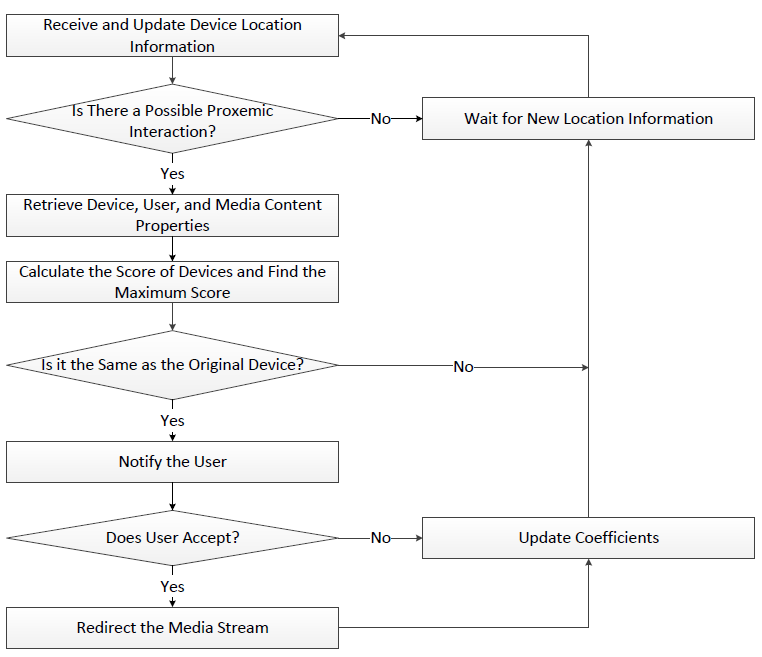
\includegraphics[width=0.8\linewidth,height=0.8\linewidth]{fig.png}
    \caption{The abstract algorithm of proxemic interaction unit.}

\end{figure}

The device scoring and recommendation step in the aforementioned algorithm is the most important step since it can assist users to engage with a larger number of devices in the IoT. To recommend the most appropriate device in the given scenario, we should find and imply different variables in the scoring mechanism. Therefore, we start by introducing these variables and then present the scoring mechanism. There are three groups involved in the proposed solution:devices, users, and multimedia content. Below we study these groups in order to find effective variables for the scoring mechanism.
\subsection{Devices}
Devices are the first and most important objects in our system. Since the proposed system provides an environment for proxemic interactions, we begin by explaining device's proximity behavior. Hall defined four perimeters around each person: intimate space, personal space, social space, and public space (Table 1) [6].We are using same categorization for devices according to their effective quality in each space: intimate devices, personal devices, social devices, and public devices. For example, smartphones have small screens, so they are usually used
by individuals separately. Moreover, they have the best visual quality when they are close to the user (e.g. 20 cm which is in the intimate space). Users can still see the smartphone screen when they are farther away, but their effective quality decreases. Similarly, users enjoy big screen TVs most when they are at an acceptable distance, i.e., 3:5 m to 6 m. Hence, they are placed in the category of public devices. Let T(x) be a function that returns an integer between 0 to 3 depending on the type of device x. Table 1 provides examples of all 4 groups of device spaces and function T() value for each device type. We will use function T() later while calculating scored for each device.

 \begin{table}[!h]
\caption{Hall's personal space definitions and device examples for each space.}
\centering
 
 \newline
\begin{tabular}{|c|c|c|c|}
	\hline
	Space Name & Sapce Area  & Device Examples & T() \\
	\hline
	Intimate Space & distance \leq 0.45\emph{m} & smartphones & 0\\
	\hline
	Personal Space & 0.45\emph{m} \leq distance \leq 1.2 \emph{m} & tablets,laptops & 1\\
	\hline
	Social Space & 1.2\emph{m} \leq distance \leq 3.6 \emph{m} & PCs, digital displays & 2\\
	\hline
	Public Space & 3.6\emph{m} \leq distance \leq 7.6 \emph{m} & TVs, home stereos & 3\\
	\hline
	
\end{tabular}
\label{t1}
\end{table}

\subsection{User Survey}
It is important to characterize user priorities in order to design effective user interface. We conducted a user survey to study user's attitudes and preferences.Participants had to answer 17 questions regarding the frequency of using multimedia contents, their device preferences, and satisfaction levels. We prepared questions such that they do not require any specific domain knowledge. Due to lack of space, we could not present the designed questionnaire here. The website we used for the study and the questionnaire details can be found at 1. Totally,149 people of an average age of 28.62 years participated in our study with the
following gender distribution: 53.7\% male and 46.3\% female. They were engineers, employees, physicians, university students and professors, etc. with different background levels in IT; 53\% of them were involved in a profession that requires a high level of IT knowledge while the other 47\% were not involved in those kinds of jobs.

Results of this user survey revealed some interesting points. First, we could not find any correlation between the gender and device preferences. However,when we grouped our participants into young and old
users, we found that old participants are more interested in using TVs and PCs than tablets and smartphones. In addition to that, profession had an effect on the device preferences. Participants who were involved in jobs that need a high level of IT knowledge were keener to use PCs and TVs. We also found that frequent users (who spend up to 1 hour per day) prefer TVs and PCs more than non-frequent users non-frequent users (who spend more than 1 hour per day).


To summarize, based on the results of this user survey, we were convinced to include three characteristics of the engaged user, u, in our scoring mechanism: participant's age ($U^a$), profession type ($U^p$), and multimedia usage habits ($U^h$).We used the user ratings to initialize preference coefficients corresponding to these characteristics, which are updated over time according to user interactions.
\subsection{Multimedia Content}
Multimedia content properties can influence the user's decision regarding the playback device. For example, a video content cannot be streamed to a home stereo, which only supports audio inputs. So, the type of the content should be considered. In addition, there is a user study that shows the length of multimedia content can affect the user's choice for playback device [18]. It categorizes videos based on their length: very short videos (up to 2 minutes, e.g. social network clips), short videos (up to 7 minutes, e.g. music videos), medium videos (up to 22 minutes, e.g. soap operas and animations), long videos (up to 45 minutes,e.g. TV series), and very long videos (longer than 45 minutes). Results of this study indicates that the length of the first half of videos that are played on the smartphones over the WiFi connection is around 50 seconds while it is almost 100 seconds for tablets. This is due to several factors such as screen dimensions and resolutions, battery capacity, etc. Hence, we decided to use three properties of the given multimedia content, c, in our scoring mechanism: audio of content ($C^a$), video of content ($C^v$), and duration of the content ($C^d$). We have grouped long and very long videos together, as a result, $C^d$ can take four values depending
on the length: 0 - very short, 1 - short, 2 - medium, and 4 - long.
\subsection{Scoring Mechnaism}
When the PIU finds out that there is a possible proxemic interaction, it starts the scoring mechanism. Let \[ \emph{D} = \big\{ D_i | 1 \leq i \leq n \big\}\]
be the set of available devices.For the given content c and a user u, the the score of $i^{th}$ device, $s_i$, is calculated
as follows:
\begin{equation}
     s_i =  f_{ic} \times m_{ic} \times h_{iu} \times a_{iu} \times p_{iu} \times d_{iu} 
\end{equation}}
where $f_{ic}$ is a flag that indicates capability of device $D_i$ to play content c, $m_{ic}$ is device appropriateness coefficient for the given content, $h_{iu}$, $a_{iu}$, and $p_{iu}$ are user's habit, age, and profession factors for the device $D_i$. The last element is $d_{iu}$ is the device effectiveness for the distance between device $D_i$ and user u. The
value of all of elements is defined between 0 and 1. We have chosen to multiply individual factor to obtain $s_i$ because for optimal results we want all factor to be unity; on the other hand, if even one factor is zero, the device is useless. For example, if a device cannot play the given content, the value of other elements do not matter at all and that device should get 0 score. In the following text,we explain each element in details.

\noindent\textbf{Playback Capability ($f_{ic}$)}This element represents the playback capability of $D_i$ for the given multimedia content c. It is a binary variable, so it is either 0 (i.e. $i_{th}$ device cannot play c) or 1 (i.e. $i_{th}$ device can play c). Equation 2 shows the Boolean expression that is used to compute $f_{ic}$:
\begin{equation}
 f_{ic} =  (D_i^a \odot C_c^a) \wedge (D_i^v \odot D_c^v)
\end{equation}}


where $D_i^a$ and $D_i^v$ logical variables which are true if device $D_i$ is capable of playing audio and video respectively, otherwise false. Similarly, $C_c^a$ and $C_c^v$ are true if the given multimedia content c has audio and video playback requirements,otherwise false.

\noindent\textbf{Device Appropriateness($m_{ic}$)}As we explained in Subsection 3.3, the length of given content ($C_c^d$) can affect the user's playback device preferences. The value of $m_{ic}$ is selected from the 44 matrix (M), which its rows represent the length of the given content and its rows show the device space types:
\begin{equation}
     m_{ic} = M(C_c^d,T(D_i))
\end{equation}}



The first row of M is dedicated to the content with length is less than 2 min, second row for the content with length between 2 min and 7 min, third row for the content with between length 7 min and 22 min, and the last row covers the rest(length is greater than 22 min). The columns follow this order: intimate devices, personal devices, social devices, and public devices. The same order is followed in the other defined matrices that have the device space type as column indicator. We defined these thresholds and matrix entries using the results of Li et al.'s survey [18] as follows:

\begin{equation}
 M =  \left[ \begin{array}{cccc}
1 & 0.8 & 0.6 & 0.4 \\
0.8 & 1 & 0.8 & 0.6\\
0.6 & 0.8 & 1 & 0.8 \\
0.4 & 0.6 & 0.8 & 1  \end{array} \right]\]
\end{equation}
\noindent\textbf{Habit ($h_{iu}$), Age ($a_{iu}$), Profession($p_{iu}$ Factors)} To determine the factors of user's multimedia usage history ($h_{iu}$), age ($a_{iu}$), and profession ($p_{iu}$);we define three binary functions as follows:


\begin{equation}
      
    U_u^h=\begin{cases}
      0, & \text{if u is a non-frequent user}  \\
      1, & \text{if u is a frequent user}
    \end{cases}
    
    U_u^a=\begin{cases}
      0, & \text{if age of u is less than 30}  \\
      1, & \text{if age of u is greater than or eqal to 30}
    \end{cases}
    
    U_u^p=\begin{cases}
      0, & \text{if u does a high IT knowledge required job}  \\
      1, & \text{otherwise}
    \end{cases}
\end{equation}

 

The factor $h_{iu}$ depends on the given user's multimedia usage habits. As we explained earlier (Subsection 3.2), user's multimedia playing time can influence the preferred playback device. The habit factor $h_{iu}$ is calculated as follows:
         \begin{equation}
             h_i^u = H(U_u^h,T(D_i))
         \end{equation}

where H is defined as a 2x4 matrix where rows represent usage frequency and columns represent device space type. The age and profession factors are also calculated in the similar way as follows:
         \begin{equation}
             a_{iu} = A(U_u^a,T(D_i))
         \end{equation}
         \begin{equation}
             p_{iu} = P(U_u^p,T(D_i))
         \end{equation}

where A and P are again 2x4 matrices.The first row of A keeps $a_{iu}$ values for users who are younger (Ua \leq 30years) and the second row presents $a_{iu}$ values for the older users. Similarly, first row of P represents users who work in a high IT knowledge required job and the second row presents rest of the users. The initial values of matrix elements of H, A, and P are determined based on user rating in the survey as follows: 
         \begin{equation}
             H =  \left[ \begin{array}{cccc}
0.8 & 0.7 & 1 & 0.9 \\
0.8 & 0.8 & 0.9 & 0.9  \end{array} \right]   A =  \left[ \begin{array}{cccc}
0.7 & 0.8 & 1 & 0.9 \\
0.8 & 0.7 & 0.9 & 1  \end{array} \right]    P =  \left[ \begin{array}{cccc}
0.8 & 0.8 & 0.9 & 1 \\
0.8 & 0.8 & 0.1 & 0.9  \end{array} \right]
         \end{equation}
         
\noindent\textbf{Distance Effectiveness($md_{iu}$)}The distance effectiveness diu is calculated using the distance between the given user u and device $D_i$. Let $x_i$ be the distance between user and device. We defined a unique device space effectiveness function for each type of device (where type is defined in terms of space). Figure 2 shows the plot of the defined functions. These functions are extracted from the obser- vations on device manuals and user's actions. For example, a big screen TV is mostly effective when.On the other hand, it is not convenient for the user to watch the TV when the distance is around 0.5 \emph{m}. You can see this behavior on the Public function in Figure 2. Similarly, user cannot clearly see a smartphone screen when too close ($x_i$ approx 0\emph{m}). However, the smartphones are very effective when xi is around 0.25 \emph{m}. Afterwards, when $x_i$ increases, their effectiveness ($d_{iu}$) decreases due to their small screen size. Generally, we can argue that the effectiveness function is asymmetric around its peak.
 \begin{figure}[h!]
    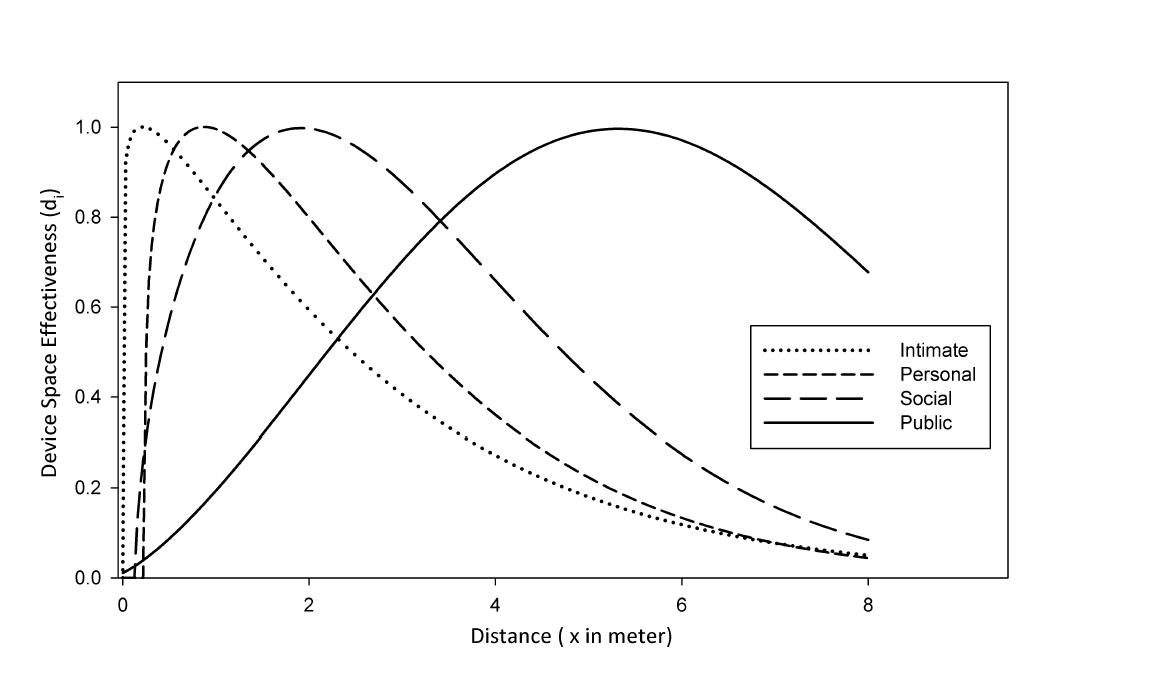
\includegraphics[width=1.0\linewidth,height=0.8\linewidth]{f1.png}
    \caption{The plot of all versions of di functions.}

\end{figure}

Finally, we could fit Weibull II with four parameters on the observed curves in order to define effectiveness function. It is restricted between 0 and 1. Equation 10 shows the general form of this function where xi is the distance between the user and device; and $x_0$, a, b, and c are four parameters, which are different for each device spaces.
 \begin{equation}
             d_i = a \times (\frac{c-1}{c})^\frac{1-c}{c} \times | \frac{x_i-x_0}{b} + (\frac{c-1}{c})^\frac{1}{c} |^{(c-1)} \times e^{-|\frac{x_i-x_0}{b}+(\frac{c-1}{c})^\frac{1}{c}|^c} + \frac{c-1}{c}  
         \end{equation}

\subsection{Adaptation Mechanism}The proposed solution considers different variables to calculate the score for each device (Equation 1) in order to find the best possible device for media redirection. Although we used the results of different surveys in order to define the values of the coefficients in the scoring mechanism, each person may have different preferences. Therefore, we designed an adaptation mechanism in the proposed solution, which updates the coefficient values based on the responses of individuals after each interaction. The PIU selects the corresponding values for coefficients and calculates the scores. For example, imagine PIU uses user's age coefficient $a_{iu}$ to calculate the score for device $D_i$, and $D_i$ is recommended to the user since it has the highest score. So, when the user responds to the recommendation, the value of $a_{iu}$ is updated using the following equation:
\begin{equation}
             a_{iu,new} = a_{iu,old} \times ( \frac{1}{1+ \frac{n_r}{n_t+1}})
         \end{equation}
where $a_{iu,new}$ is the new coefficient's value, $a_{iu,old}$ is the old coefficient, $n_r$ is number of rejected recommendations for this type of device space, and $n_t$ is the total number of recommendations for this type of device space.
\section{Evaluation}
To evaluate the proposed system, we defined 4 scenarios and conducted a user survey. In these scenarios, participants were given access to all types of devices in their effective distance. The content's length was the only variable in our scenarios. In the first scenario, it was 2 min while it was 7 min, 22 min, and 90 min in the second, third and fourth scenarios respectively. As an example, the user had to select his / her preferred device for watching a 7 min video while he / she has access to a smartphone in 0.25 m, tablet in 0.75 m, personal computer in 2.5 m, and TV in 5 m. Totally, 10 people participated in our study with age ranging from 20 to 40. The users had different professions and media playback habits. We compared the user responses to the device recommendations made
by the proposed user interface to measure the usability.
We also compare the proposed approach with two other methods. The first
one only uses the distance to suggest a new device. So, the method always suggests the device that has user in its most effective area, with the same learning mechanism as ours. The second method is AirPlayer [17]. AirPlayer only supports intimate and public devices. Furthermore, it does not have the learning mechanism. So, it cannot adapt itself to user's preferences.
Table 2 shows the results of this evaluation study.


\begin{table}[!h]
\caption{The results of the evaluation study.}
\begin{tabular}{@{}llllll@{}}
\cmidrule(r){1-2}
\multicolumn{2}{|c|}{\textbf{method}}                                                           & scenario 1 & scenario 2 & scenario 3 & scenario 4 \\ \cmidrule(r){1-2}
\multirow{2}{*}{\begin{tabular}[c]{@{}l@{}}our \\ method\end{tabular}}     & 1st suggestion      & 90\%       & 30\%      & 70\%      & 90\%      \\
                                                                           & 1st/2nd suggestion & 100\%      & 80\%      & 80\%      & 100\%     \\
\multirow{2}{*}{\begin{tabular}[c]{@{}l@{}}Distance\\   only\end{tabular}} & 1st suggestion     & 90\%       & 30\%      & 60\%      & 90\%      \\
                                                                           & 1st/2nd suggestion & 100\%      & 70\%      & 70\%      & 100\%     \\
AirPlayer{[}17{]}                                                          & -                  & 100\%      & 30\%      & 30\%      & 90\%     
\end{tabular}
\end{table}
In this study, the total accuracy of the rst suggestion for our system is
equal to 70\% while it was 67.5\% for the distance only method and 62.5\% for the
AirPlayer. But, since the proposed method can learn from the users responses and adapt itself to his / her preferences, we decided to study the accuracy of these methods after two interactions. This is not applicable to the AirPlayer due to its lack of learning mechanism. The total accuracy after two interactions for our system was 90\%, however it was 85\% for the distance only method. To summarize, we can say that the proposed method had a higher accuracy in these scenarios. As a result, it could provide an environment that has more successful proxemic multimedia interactions.

\section{Discussion}
There are three points that should be discussed regarding the proposed system.First, the proposed solution checks the identity of users by tracking their intimate devices. Then, it uses their personal information to recommend a device to them and adaptively updates itself for each user. Also, each device or user updates the location information when it has a movement. The devices are recommended based on the distance between them. Therefore, we can conclude that the proposed solution directly uses 3 out of 5 proxemic interaction dimensions that were introduced earlier by Greenberg et al [7]. The remaining two dimensions can be involved in this system as well. The orientation of the user and location of devices may influence the user's decision on playback device.

Second, we should compare the proposed UI with the definition of proxemic
interaction by Hall [6]. The proposed UI is designed to work over the IoT. So,it can handle proxemic interactions in multiple rooms (i.e. macro-level). But it provides an environment for micro-level proxemic interactions as well. Devices within a single room can interact with each other when a measured change occurs in any of the 3 mentioned proxemic dimensions.

The last point is regarding the engagement mechanism. Since the number
of online devices is growing very fast, most of the times users are surrounded by a number of devices. But, since it is not easy to migrate from one device to the other, users may not change the device that they are using. However, the proposed UI considers the user's preferences and proxemic information to suggest a new device, which can increase the number of accepted recommendations. Also, it can assist users through the migration process by handling redirection process in the background. Hence,the proposed UI facilitates the engagement process for the users and provides them more options to use.
\section{Conclusion and Future Work}This paper presented a new UI, which is designed for multimedia devices within the IoT. The proposed UI provides a proxemic interaction experience to the users. The proposed solution involves user's preferences and media content properties in addition to the proxemic information in its scoring mechanism. Then, it recommends a new device to the user in order to motivate him/her to engage with the new device. The proposed algorithm adaptively trains itself towards user's attitude over the time based on the feedback from the user. The scoring
mechanism is validated in 4 scenarios by a user study and it has the acceptable average accuracy of 70\%. Using the feedback from the rejection ratio, system trains itself towards user's attitude over the time and reaches average accuracy of 90\%. In the future, we want to include more devices and interaction modalities to build a generic, distributed user interface for IoT.














\section{References}
\begin{enumerate}


    \item \textit Sanou, B.: ICT Facts and Figures. International Telecommunications Union, Geneva(2013)
    \item \textit Mattern, F., Floerkemeier, C.: From the Internet of Computers to the Internet of Things. In: From active data management to event-based systems and more, pp.242-259. Springer, Heidelberg (2010)
    \item \textit Connections Counter: The Internet of Everything in Motion, http://newsroom. cisco.com/feature-content?type=webcontent&articleId=1208342
    \item \textitWeiser, M.:, The computer for the 21st century. In: Scientic American, pp. 94-104
(1991)
    \item \textitLuyten, K., Coninx, K.: Distributed user interface elements to support smart inter-
action spaces. In: 7th IEEE International Symposium on Multimedia, pp. 277-286.
IEEE Press, New York (2005)
    \item \textit Hall E.T.: The hidden dimension. Anchor Books, New York (1969)
    \item \textit Greenberg, S., Marquardt, N., Ballendat, T., Diaz-Marino, R., Wang, M.: Proxemic
interactions: The new ubicomp?. Interactions. 18(1), 42{50 (2011)
    \item \textit  Marquardt, N., Diaz-Marino, R., Boring, S., Greenberg, S.: The proximity toolkit:
Prototyping proxemic interactions in ubiquitous computing ecologies. In: 24th Annual ACM Symposium on User Interface Software and Technology, pp. 315{326.ACM, New York (2011)
    
    \item \textit  Kortuem, G., Kawsar, F., Fitton, D., Sundramoorthy, V.: Smart objects as building blocks for the internet of things. Internet Computing,IEEE. 14(1), 44{51 (2010) 
    
    \item \textit Broll, G., Rukzio, E., Paolucci, M., Wagner, M., Schmidt, A., Hussmann, H.: Perci: Pervasive service interaction with the internet of things. Internet Computing,IEEE. 13(6), 74{81 (2009)
    \item \textit Guinard, D., Trifa, V.: Towards the web of things: Web mashups for embedded devices. In: MEM 2009 in Proceedings of WWW 2009, ACM, New York (2009)
    \item \textit Ju, W., Lee, B.A., Klemmer, S.R.: Range: Exploring implicit interaction through
electronic whiteboard design. In: the 2008 ACM Conference on Computer Supported Cooperative Work, pp. 17{26. ACM, New York (2008)
    \item \textit Wang, M., Boring, S., Greenberg, S.: Proxemic peddler: A public advertising dis-
play that captures and preserves the attention of a passerby. In: the 2012 International Symposium on Pervasive Displays, pp. 3:1{3:6. ACM, New York (2012)
    \item \textit Want, R., Hopper, A., Falc ao, V., Gibbons, J.: The active badge location system.ACM J. Transactions on Information Systems 10(1), 91{102 (1992)
    \item \textit  Brumitt, B., Meyers, B., Krumm, J., Kern, A., Shafer, S.A.: Easyliving: Technologies for intelligent environments. In: 2nd International Symposium on Handheld and Ubiquitous Computing, pp. 12{29. Springer-Verlag, London (2000)
    \item \textit Ramani, I., Bharadwaja, R., Rangan, P.V.: Location tracking for media appliances in wireless home networks. In: IEEE International Conference on Multimedia and Expo, pp. 769{772. IEEE Press, New York (2003)
    \item \textit Srensen, H., Kristensen, M.G., Kjeldskov, J., Skov, M.B.: Proxemic interaction in a multi-room music system. In: 25th Australian Computer-Human Interaction Conference: Augmentation, Application, Innovation, Collaboration, pp. 153{162. ACM, New York (2013)
    \item \textit Li, Z., Lin, J., Akodjenou, M.I., Xie, G., Kaafar, M.A., Jin, Y., Peng, G.: Watching Videos from Everywhere: A Study of the PPTV Mobile VoD System. In: the 2012 ACM Conference on Internet Measurement Conference, pp. 185{198. ACM, New York (2012)
    
    
    
    
    
\end{enumerate}}


\end{document}